\documentclass[a4paper]{ltxdoc}

\usepackage{ocg-p}
\usepackage{tikz}
\usetikzlibrary{arrows,automata}
\usepackage{color}

\newcommand*{\pkg}[1]{\textsf{#1}}

\title{\pkg{OCG-P} package, example 3}

\begin{document}

\maketitle

\section{Text layers changed by clicking on a link element}
The following text can be toggled: 
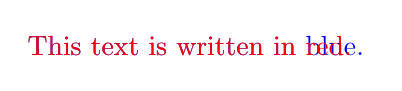
\begin{tikzpicture}[baseline=0]
\tikzstyle{nome}=[anchor=base,outer sep=0,inner sep=0,minimum height=.45cm,minimum width=4.4cm]
\begin{ocg}{blue text}{ocblueid}{1}
  \node[nome,blue]        (p1)  {\parbox[b][][t]{4.4cm}{This text is written in blue.}};
\end{ocg}
\begin{ocg}{red text}{ocredid}{0}
  \node[overlay,nome,red] (p2)  {\parbox[b][][t]{4.4cm}{This text is written in red.}};
\end{ocg}
\end{tikzpicture}
And now the text is black again.\\

\toggleocgs{ocblueid ocredid}{Click here to toggle the text!}



\section{Mouseover example}

Make the text visible by moving the mouse in the box around.

\fbox{
\begin{ocg}{This}{octhis}{0}
 \toggleocgs[triggerocg=allactions]{octhis, octhis}{This}
\end{ocg}
\begin{ocg}{text}{octext}{0}
 \toggleocgs[triggerocg=allactions]{octext, octext}{text}
\end{ocg}
\begin{ocg}{is}{ocis}{0}
 \toggleocgs[triggerocg=allactions]{ocis,ocis}{is}
\end{ocg}
\begin{ocg}{not}{ocnot}{0}
 \toggleocgs[triggerocg=allactions]{ocnot, ocnot}{not}
\end{ocg}
\begin{ocg}{visible}{ocvisible}{0}
 \toggleocgs[triggerocg=allactions]{ocvisible, ocvisible}{visible.}
\end{ocg}
}



\end{document}